\section{Dataset}

The Cityscapes dataset is a large-scale dataset widely used for training and evaluating algorithms in the fields of computer vision, particularly for semantic understanding of urban street scenes. It consists of high resolution images captured from a vehicle-mounted camera while driving through various cities in Germany, including Frankfurt, Munich and Strasbourg. The capturing apparatus that was used was equipped with a dual for stereoscopic capability, allowing for the possibility of applying stereo vision techniques useful for tasks like depth estimation, 3D reconstruction and scene understanding. 

The images that are used in our analysis are located in the folder \textbf{leftImg8bit}. These are taken from the left camera of the stereo camera system. These are the main high-resolution images (2048 $\times$1024 pixels) with an 8-bit color depth that are used for all semantic and instance segmentation tasks. Each image is stored in a PNG file format with a size that varies between 2.0 and 2.5 MB. The images have an RGB color space, which means that there are 3 color channels for each image.

The dataset includes two different types of image annotations:\\
\textbf{Fine annotations:} These provide detailed, pixel-level annotations for 5,000 images which have labels for 30 classes such as road, car, pedestrian, building, and traffic light. This dataset is split into 2,975 annotations for training, 500 for validation and 1,525 for testing (see Figure \ref{fig:cityscapes}(b)). It is worth mentioning that the ground truth annotations are not available to the users and this happens in order to allow for fair evaluation and benchmarking of models. Users instead need to submit their code to an online evaluation server which provides the quantitative performance metrics.    

\textbf{Coarse annotations:} These include a much larger set of 20,000 images with less precise annotations intended for data augmentation and for tasks where granularity is not critical (see Figure \ref{fig:cityscapes}(a) for an example). The coarse annotations are split into a training and validation set. No test set is provided since this is only done using the fine annotations set. 

\begin{figure}[ht]
    \centering
    \begin{subfigure}{0.45\textwidth}
        \centering
        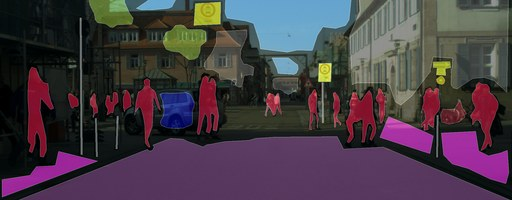
\includegraphics[width=\linewidth]{coarse_example.jpg}
        \caption{Coarse mask}
        \label{fig:sub1}
    \end{subfigure}\hfill
    \begin{subfigure}{0.45\textwidth}
        \centering
        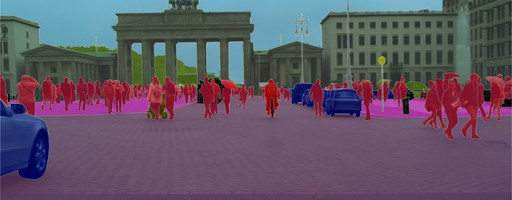
\includegraphics[width=\linewidth]{fine_example.jpg}
        \caption{Fine mask}
        \label{fig:sub2}
    \end{subfigure}
    \caption{Examples of coarse (a) and fine (b) mask annotations superimposed on the corresponding original images}
    \label{fig:cityscapes}
\end{figure}

The scenes in our dataset represent a variety of urban settings, seasons, daylight conditions, and weather scenarios, providing robust, real-world environments for training models that need to perform under varied conditions. This dataset has been widely used in research for developing and testing algorithms on tasks such as object detection, semantic segmentation, and instance segmentation in urban settings as well as advancing the state-of-the-art in visual perception for autonomous driving systems. The Cityscapes dataset can be accessed in the following address:
\begin{center}
\url{https://www.cityscapes-dataset.com}
\end{center}
Our particular approach in this study is to create and train at least two models; one with a basic architecture that will form our baseline and a second one where we will be exploring a more complex architecture. We are aiming to demonstrate first of all that both our models are able to perform semantic segmentation on the chosen dataset. Our second goal is to investigate how the choice of various hyper-parameters and tweaks in architecture can affect the accuracy and performance of the models. 
